\documentclass{article}
\usepackage{graphicx} % Required for inserting images
\usepackage{booktabs}
\usepackage{hyperref}
\hypersetup{
    urlcolor=cyan,
    linkcolor=blue,
    colorlinks=true,
    pdftitle={Rapport Projet BDR Thermea},
    pdfpagemode=FullScreen,
    }
\usepackage{float}
\usepackage{listings}
\usepackage{amsmath}
\usepackage{array}
\usepackage{amsmath}
\usepackage{amssymb}
\usepackage{centernot}
\usepackage{algpseudocode}
\usepackage{stmaryrd}
\usepackage{tikz}
\usepackage{subfigure}
\usepackage{mathtools, stmaryrd}
\usepackage{xparse} \DeclarePairedDelimiterX{\Iintv}[1]{\llbracket}{\rrbracket}{\iintvargs{#1}}
\NewDocumentCommand{\iintvargs}{>{\SplitArgument{1}{,}}m}
{\iintvargsaux#1} %
\NewDocumentCommand{\iintvargsaux}{mm} {#1\mkern1.5mu..\mkern1.5mu#2}
\usepackage{pgfplots}
% \pgfplotsset{compat=1.18}
\usepackage[french]{babel}

\title{BDR Thermea: Modèle 3D d'une hélice toroïdale}
\author{Sacha Alidadi Heran}
\date{\today}

\begin{document}

\maketitle

\tableofcontents

\newcommand{\diam}{\text{diam}}

\section{Introduction}

\subsection{Présentation de l'entreprise}

BDR Thermea est un leader mondial en matière de solutions de chauffage intelligentes. Cette entreprise est née en 2009 de la fusion de 3 entreprises Baxi, De Dietrich, Remeha.

Elle est connue pour ses solutions de chauffage et d'eau chaude, fournissant des produits à travers l'Europe de l'Ouest, notamment au Royaume-Uni, en France, en Allemagne, en Espagne, aux Pays-Bas et en Italie.

L'entreprise se distingue par ses chiffres impressionnants. Chaque année, 1,4 million d'utilisateurs finaux choisissent les produits de BDR Thermea. Elle emploie plus de 6 100 personnes et ses produits sont vendus dans plus de 100 pays, générant un chiffre d'affaires de 2,1 milliards d'euros.

BDR Thermea se compose de plusieurs marques à travers le monde, y compris Baxi, De Dietrich, Remeha, Brötje, Chappee, Sofath, Oertli, Baymak, Heatrae Sadia, Megaflo, et Potterton.

Au sein de cette entreprise, le projet se déroulera au département Business Development Unit chargé des simulations.

\subsection{Contexte}

Les ingénieurs de BDR Thermea France, en particulier ceux travaillant sur les pompes à chaleurs, cherchent à réduire le bruit généré par l'Outdoor Unit (Unité extérieure de la pompe à chaleur). On sait que le ventilateur à l'intérieur de l'unité est à l'origine du bruit.

Une étude du MIT \href{https://www.ll.mit.edu/sites/default/files/other/doc/2023-02/TVO_Technology_Highlight_41_Toroidal_Propeller.pdf}{[1]} a montré que donner une forme toroïdale aux hélices d'un drone permet de réduire le bruit généré par ce dernier. La forme des hélices est représentée sur la figure \ref{fig:Propeller}

\begin{figure}[H]
    \centering
    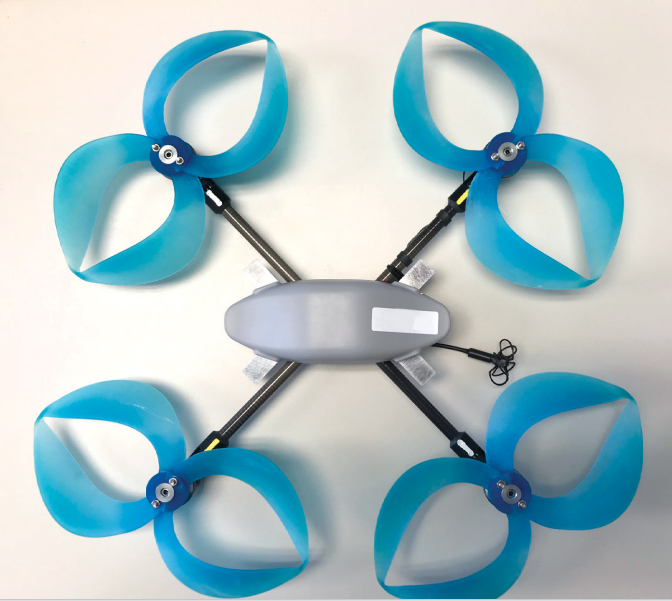
\includegraphics{images/ToroidalPropeller.png}
    \caption{Drone avec des hélices en forme toroïdale}
    \label{fig:Propeller}
\end{figure}

La figure \ref{fig:GraphSound} montre un graphique comparatif du bruit généré par une hélice avec une forme normale et une forme toroïdale. L'abscisse représente la fréquence du bruit et l'ordonnée représente la pression en dBA.

\begin{figure}[H]
    \centering
    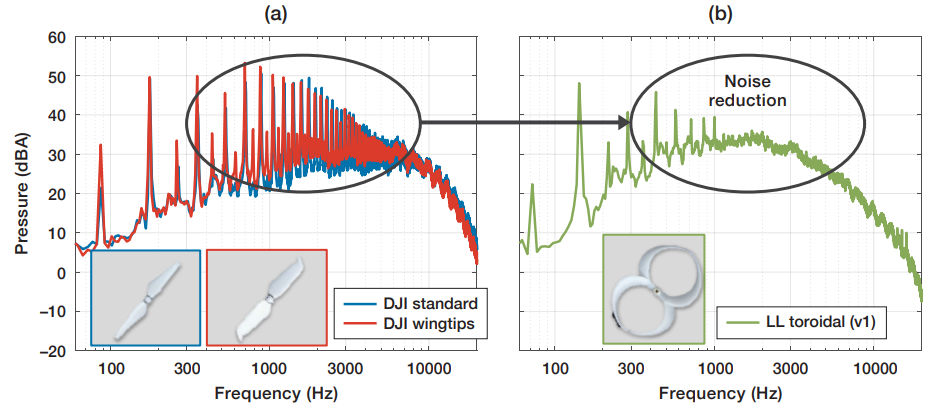
\includegraphics{images/NormalVSToroidal.png}
    \caption{Graphique comparant le bruit entre une hélice avec une forme normale et une forme toroïdale.}
    \label{fig:GraphSound}
\end{figure}

Le graphique montre une diminution significative du bruit tonal (Les bruits correspondant au pic dans le graphique) avec les hélices à forme toroïdale. Ainsi, les ingénieurs de BDR Thermea veulent vérifier si un ventilateur en forme toroïdale permettra de réduire le bruit de l'Unité extérieure de la PAC (Pompe à chaleur).

\subsection{Objectifs}

Comme il y a peu de documentation autour des hélices toroïdales pour le moment, ce projet a deux objectifs:

\begin{itemize}
    \item Établir les expressions mathématiques permettant de générer la courbe guide et les profiles transverses
    \item Écrire une routine de generation de géométrie 3D paramétrée dans un logiciel OpenSource (SALOME)
\end{itemize}

\subsection{Modifications de la roadmap}

\label{sec:Roadmap}

Au début, du projet, une roadmap a été établie pour mener à bien le projet. La roadmap est affichée sur la figure \ref{fig:RoadmapV0}

\begin{figure}[H]
    \centering
    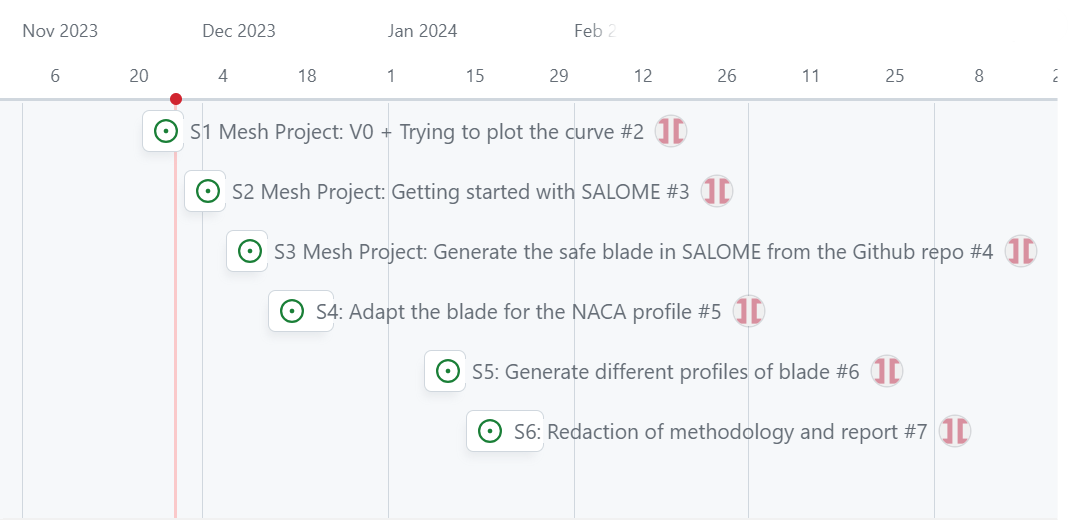
\includegraphics[scale=0.75]{images/RoadmapV0.png}
    \caption{Roadmap du projet}
    \label{fig:RoadmapV0}
\end{figure}

Semaine 1: Rendu de la V0 + Afficher la courbe

Pour faire la V0 (Rapport + Présentation), il a fallu commencer par étudier la documentation existante. En particulier deux références autour des hélices toroïdales

\begin{itemize}
    \item Mathematical expression method for geometric shape of toroidal propeller, YE Liyu, WANG Chao, SUN Cong, GUO Chunyu, 2023 \href{http://www.ship-research.com/cn/article/doi/10.19693/j.issn.1673-3185.03419}{[2]}
    \item Toroidal propeller generator \href{https://github.com/RaulBejarano/Ultimate-Toroidal-Propeller-Generator}{[3]}
\end{itemize}

Le premier document est un papier sur les équations d'une hélice de bateau à forme toroïdale. Les équations du document présentent un inconvénient, c'est qu'elles sont adaptées seulement pour des hélices de bateau. Cependant, elles ont l'avantage de prendre en compte le profil NACA (profil aérodynamiques).

Le second document est un repository github contenant un fichier .scad permettant de générer des modèles 3D d'hélices toroïdales. 
La forme des modèles correspond aux hélices recherchées, cependant la manière dont sont générés les modèles ne convient pas aux besoins du projet.
En effet, la manière dont sont générés les pales ne les rendent pas aérodynamiques. Ce problème sera abordé dans la section \ref{sec:HeliceToroCAD}

Le résultat donne une pale avec un profil avec des bords irréguliers ce qui n'est pas adapté aux hélices de PAC.

Semaine 2: Prise en main de SALOME

Pour mener à bien ce projet, il a fallu utiliser le logiciel SALOME. C'est pourquoi il fallait suivre des tutoriels venant du site SALOME pour prendre en main cet outil

Semaine 3: Générer une pale en forme toroïdale sur SALOME

Dans le repository github, le fichier permettant de générer les hélices est un fichier .scad qui est destiné au logiciel "OpenSCAD". Il était donc nécessaire de recréer les pales de ce fichier sur SALOME.

Semaine 4: Adapter le profil des pales

Une fois les pales générées, il fallait les modifier pour les rendre aerodynamiques. Pour cela, des profils NACA ont été utilisés. Les profils NACA seront détaillés dans la section \ref{sec:HeliceToroMath}

Semaine 5: Générer différentes géométries de ventilateurs

Pour savoir si des hélices toroïdales permettent de réduire le bruit de la PAC, il a fallu générer différents profils d'hélices. Pour ça, les paramètres géométriques des hélices ont été modifiés.

Semaine 6: Écriture de la méthodologie et du rapport

Pour que les modèles d'hélices soit réplicables par les employés de BDR Thermea en vue des simulations, une méthodologie pour générer ces modèles a été créée sous la forme d'un fichier README.md. Cela inclut entre autres, les équations et les fichiers géométriques.

\vspace{1cm}

Durant le projet, la roadmap a du être modifiée. En particulier la semaine 4 a du être modifiée. En effet, il s'agit d'un projet d'innovation, ce qui a amené la roadmap à être conçue de telle sorte que différentes approches ont été testées. En particulier, deux approches ont été testées:

\begin{itemize}
    \item Une approche mathématique
    \item Une approche CAO (\href{https://fr.wikipedia.org/wiki/Conception_assist%C3%A9e_par_ordinateur}{Conception Assistée par Ordinateur})
\end{itemize}

La première semaine a montré qu'une approche mathématique pour générer des hélices toroïdales est possible. Par conséquent, la roadmap a été modifiée pour que le projet se concentre sur la création d'une équation mathématiques des courbes guides. Cependant, la fin du projet approchant et l'établissement des équations prenant plus de temps que prévu, la fin du projet a finalement porté sur une approche CAO. Les résultats de l'approche mathématique seront détaillés dans la section \ref{sec:HeliceToroMath} et les résultats de l'approche CAO dans la section \ref{sec:HeliceToroCAD2}.

\section{Contributions}

\subsection{Équations paramétriques d'une hélice toroïdale d'un bateau}

%% Add a label to reference it later

\hypertarget{Modele1}{Au} cours de la première semaine, l'attention a été portée sur l'étude des équations paramétriques relatives à l'hélice toroïdale d'un bateau. Cette analyse a permis de générer à la fois la courbe guide et les profils transverses de ladite hélice.

La figure \ref{fig:CourbeGuide} montre la courbe guide de l'hélice toroïdale d'un bateau.

\begin{figure}[H]
    \centering
    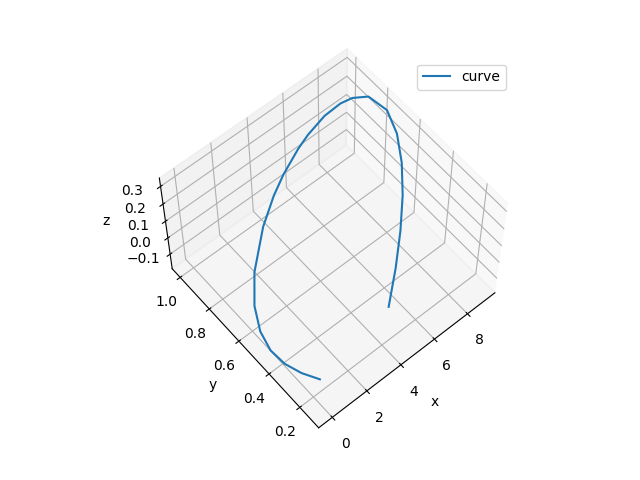
\includegraphics{images/Curve1D.png}
    \caption{Courbe guide de l'hélice toroïdale d'un bateau}
    \label{fig:CourbeGuide}
\end{figure}

La courbe ci-dessus a été généré à partir de l'équation suivante dont les paramètres seront détaillés juste après

$\begin{cases}
    x = l + x_T +\left( \frac{-b}{2}+s \right) \sin\beta + \begin{pmatrix}
        y_b \\
        y_f
    \end{pmatrix} \cos\beta \\
    r = r_l \\
    \theta = \phi + \theta_s + \frac{1}{r} \left[ \left( \frac{-b}{2}+s \right) \cos\beta + \begin{pmatrix}
        y_b \\
        y_f
    \end{pmatrix} \sin\beta \right]
\end{cases}$

Où:

$l$ représente le paramètre variant entre $0$ et $1$.

$x_T$ est la valeur totale de l'inclinaison, composée principalement de deux parties, la valeur de l'inclinaison de la lame elle-même et la valeur de l'inclinaison causée par l'obliquité. L'équation suivante explique comment calculer $x_T$

\[ x_T(r) = x_l(r)+r \theta_s(r) \tan \beta(r) \]

$x_l$ représente l'inclinaison au niveau de la section de la lame.

$\beta$ représente l'angle de calage géométrique à un certain rayon $r$, indiquant le degré d'inclinaison de la section de la pale à ce rayon.

$b$ est le diamètre du profil transverse.

$s$ est la distance entre un point du profil de la pale et le générateur. Voici un schéma expliquant ce paramètre:

\begin{figure}[H]
    \centering
    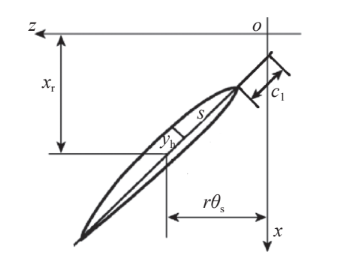
\includegraphics{images/ProfilTransverse.png}
    \caption{Profil transverse d'une pale}
    \label{fig:ProfilTransverse}
\end{figure}

$ \begin{pmatrix}
    y_b \\
    y_f
\end{pmatrix}$, aussi noté $y_h$ représente la hauteur du profil de la pale.

Enfin, $\theta_s$ représente la distribution de l'angle oblique.

De plus, l'équation est représentée en coordonnées cylindriques avec la particularité d'avoir comme coordonnées $(x,r,\theta)$. En général, les coordonnées cylindriques s'écrivent sous la forme $(z,r,\theta)$. Dans le cas des hélices toroïdales, $x$ représente la coordonnée en abscisse, $r$ représente le module du point projeté sur le plan $0yz$, et theta l'angle par rapport à l'axe $x$ du point projeté sur le plan $0yz$.

Une fois l'équation de la courbe guide établie, il faut générer un profil transverse. La figure suivante montre le profil transverse généré à partir de l'équation présentée dans le papier:

\begin{figure}[H]
    \centering
    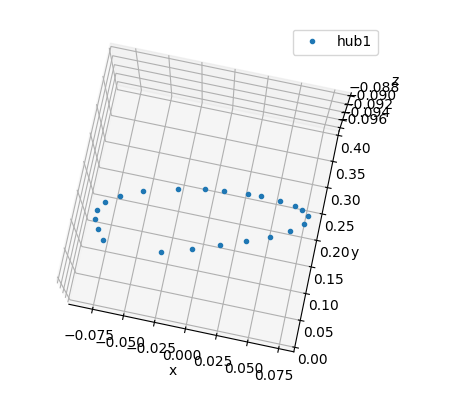
\includegraphics{images/Transverse_profile_fan_chinese_paper.png}
    \caption{Profil transverse généré à partir de l'équation ci-dessous}
    \label{fig:ProfilPale}
\end{figure}

L'équation suivante est celle présentée dans le papier:

$ \begin{cases}
    x = x_l + r \theta_s + \tan(\beta) \\
    y = r \cos(\theta) \\
    z = r \sin(\theta)
\end{cases} $

Les paramètres dans cette équation sont identiques à ceux de la courbe guide. Il y a seulement un nouveau paramètre $\theta$ qui représente l'angle par rapport à l'origine du point projeté sur le plan $0yz$. Ici, il vaut 0.

\vspace{0.5cm}

Maintenant que la courbe guide et le profil transverse ont été générées, l'hélice toroïdale peut être générée. Pour ça, il faut utiliser le logiciel SALOME qui permet d'extruder une face comme le profil transverse le long d'une courbe guide. La figure \ref{fig:HeliceToroBoat} montre le résultat de l'extrusion de la face:

\begin{figure}[H]
    \centering
    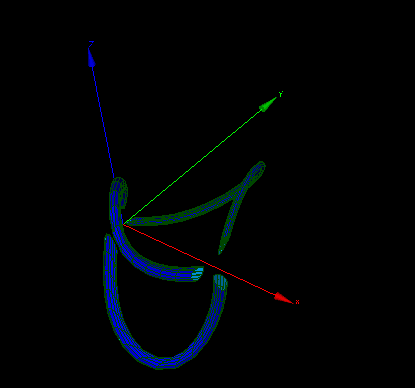
\includegraphics{images/ToroidalPropellerBoat.png}
    \caption{Hélice toroïdale d'un bateau}
    \label{fig:HeliceToroBoat}
\end{figure}

Les courbes guides peuvent également être projetées sur le plan $0yz$ pour avoir une variante de l'hélice toroïdale. Concrètement cela revient à mettre $x=0$ dans l'équation de la courbe guide. La figure \ref{fig:HeliceToroBoat2} montre le résultat de la projection:

\begin{figure}[H]
    \centering
    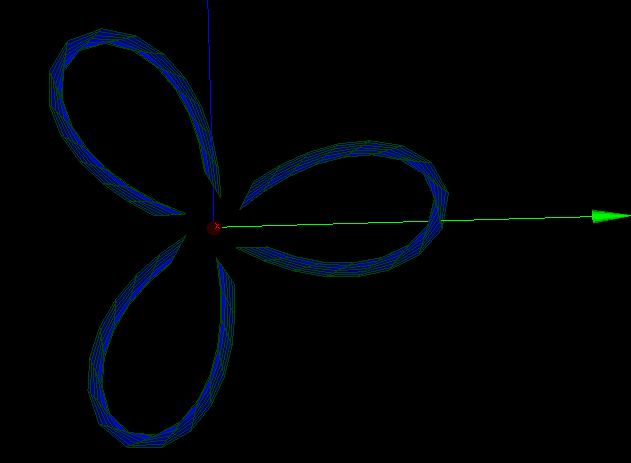
\includegraphics{images/ToroidalPropellerBoatProjected.png}
    \caption{Hélice toroïdale d'un bateau projeté sur le plan $0yz$}
    \label{fig:HeliceToroBoat2}
\end{figure}

Ces équations, bien qu'intéressantes, présentent un souci majeur, les paramètres ne peuvent pas être modifiés. En effet, le papier utilisé donne les paramètres géométriques mais n'explique pas comment les calculer. Il a donc fallu trouver une autre méthode pour générer des hélices toroïdales. En particulier, il faudrait trouver une équation reprenant les paramètres importants de l'équation précédente et qui puissent être calculés. Les paramètres choisis sont les suivants:

\begin{itemize}
    \item La largeur de la pale
    \item La hauteur de la pale
    \item L'angle d'inclinaison de la pale
    \item Le nombre de pales
    \item La distance selon l'axe $z$ entre le point de départ de la courbe guide et le point de fin de la courbe guide
\end{itemize}

Une telle équation a pu être trouvée, elle sera détaillée dans la section \ref{sec:HeliceToroMath}.

\subsection{Hélice toroïdale en CAO}

\label{sec:HeliceToroCAD}

\hypertarget{Modele2}{Le} deuxième document mentionné est un repository github contenant un fichier .scad permettant de générer des modèles 3D d'hélices toroïdales. La forme globale des modèles correspond à ce qui est souhaité, cependant le profil des pales ne convient pas à un ventilateur pour PAC. En effet, les pales sont générées à partir d'une extrusion de cercle, ce qui lui donne une forme trop angulaire. Or ce qui est recherché, ce sont des pales avec un profil NACA. De plus, l'hélice a été générée sur OpenSCAD, un logiciel de CAO. Il a donc fallu recréer les pales sur SALOME.

Pour cela, une analyse du fichier .scad s'imposait afin de comprendre comment les pales étaient générées. Les étapes pour générer une telle hélice sont expliquées ci-dessous:

\begin{itemize}
    \item Génèrer deux cercles concentriques
    \item Génèrer une couronne entre les deux cercles
    \item Extruder la couronne le long d'une courbe guide (Ici il s'agit d'un segment de droite avec une pente de 45 degrés)
    \item Effectuer une rotation de la couronne autour de l'axe $z$ (L'angle de la rotation dépend du nombre de pales)
    \item Gérer les intersections entre les pales
\end{itemize}

La figure ci-dessous montre le résultat de ces étapes en prenant 3 pales:

\begin{figure}[H]
    \centering
    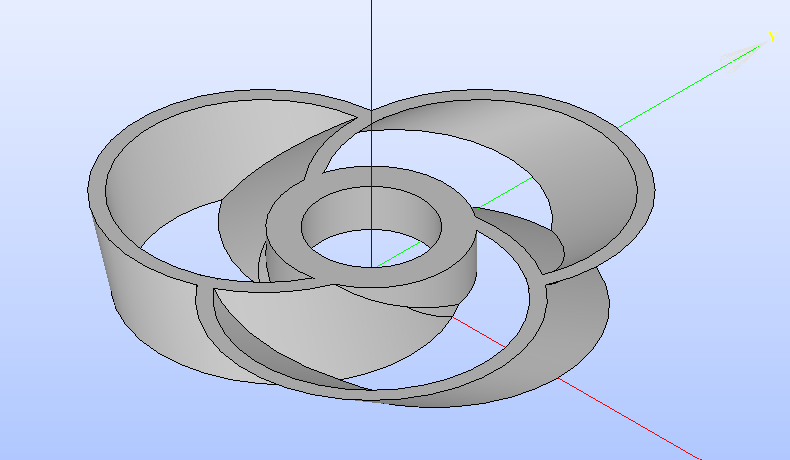
\includegraphics{images/ToroidalPropellerCAD.png}
    \caption{Hélice toroïdale générée sur OpenSCAD}
    \label{fig:HeliceToroOpenSCAD}
\end{figure}

\begin{figure}[H]
    \centering
    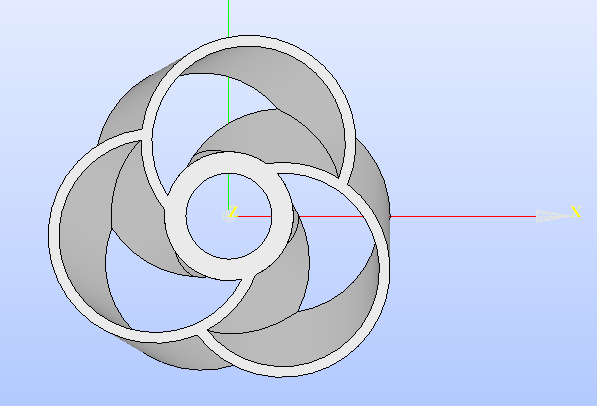
\includegraphics{images/ToroidalPropellerCADTopView.png}
    \caption{Vue de dessus de l'hélice toroïdale générée sur OpenSCAD}
    \label{fig:HeliceToroOpenSCAD2}
\end{figure}

Puisque ces hélices n'ont pas de profil NACA, et que les équations du premier document sont encourageantes. Il était nécessaire de corriger la roadmap comme mentionné précédemment afin de consacrer plus de temps sur l'écriture des équations mathématiques. Ce qui a abouti à une nouvelle équation qui sera détaillée dans la section suivante \ref{sec:HeliceToroMath}.

\subsection{Équations paramétriques d'une hélice toroïdale adaptée à une pompe à chaleur}

\label{sec:HeliceToroMath}

\hypertarget{Modele3}{Pour} trouver une équation satisfaisante, \href{https://mathcurve.com/}{ce site} répertoriant des courbes paramétrées s'est avéré utile. Parmi les courbes trouvées, la quadrifolium et la trifolium ont été choisies. Ce sont des courbes très simples qui, comme comme leur nom l'indique, représente un trèfle à quatre ou trois feuilles. L'équation suivante permet de générer la trifolium en 2D:

$ \begin{cases}
    x(t) = \cos(2t) - \cos(t) \\
    y(t) = \sin(2t) + \sin(t)
\end{cases} $

Dans la suite du rapport, cette équation sera utilisée pour générer des courbes paramétrées, car elle peut être généralisée pour générer des quadrifoliums, pentafoliums, etc. La figure \ref{fig:Trifolium} montre la trifolium générée avec cette équation:

\begin{figure}[H]
    \centering
    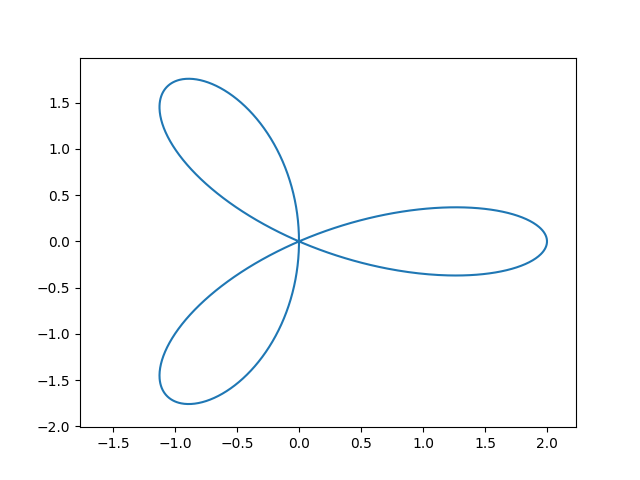
\includegraphics[scale=0.65]{images/Trifolium.png}
    \caption{Courbe 2D de la trifolium}
    \label{fig:Trifolium}
\end{figure}

L'inconvénient de cette courbe est qu'elle est en 2D. Il va donc falloir lui ajouter une troisième dimension. De plus, il faut inclure des paramètres géométriques pour pouvoir générer des hélices toroïdales. Dans le cas du projet, les paramètres suivants ont été retenus:

\begin{itemize}
    \item L'angle d'inclinaison de la pale $\theta$
    \item Le nombre de pales $N$
    \item La hauteur de la courbe guide $h$
    \item La distance entre le point de départ et d'arrivée de la courbe guide $L$
\end{itemize}

Avec ces paramètres, l'équation 3D suivante permet de générer une courbe guide:

$ \begin{cases}
    x(t) = \cos((N-1)t) - \cos(t) \\
    y(t) = \sin((N-1)t) + \sin(t) \\
    z(t) = \sin(Nt)\theta + \left\{ \frac{t N}{2\pi} \right\} L
\end{cases} $

Avec $\{ x \}$, la partie fractionnaire de $x$.

De plus, le paramètre $h$ n'apparaît pas dans l'équation car il sera inclus plus tard en effectuant l'opération suivante:

$ \begin{cases}
    x(t) = \frac{x(t)h}{\diam(\mathcal{C})} \\
    y(t) = \frac{y(t)h}{\diam(\mathcal{C})} \\
\end{cases} $

Où $\mathcal{C}$ est la courbe guide et $\diam(\mathcal{C})$ est le diamètre de la courbe guide qui se calcule ainsi:

\[ \diam(\mathcal{C}) = \max_{t \in [0,2\pi]} \sqrt{x(t)^2+y(t)^2} \]

\vspace{0.5cm}

Maintenant, il faut expliquer d'où viennent les termes dans $z(t)$. $z(t)$ est composé de deux termes importants

\begin{itemize}
    \item $\sin(Nt) \theta$ qui permet d'incliner la courbe guide pour chaque pale.
    \item $\left\{ \frac{t N}{2\pi} \right\} L$ qui permet de décaler le point de départ et d'arrivée de la courbe guide selon l'axe $z$.
\end{itemize}

Plus $\theta$ est grand, plus la pale sera inclinée. Plus $L$ est grand, plus la courbe guide sera décalée selon l'axe $z$.

\vspace{0.5cm}

Maintenant que la courbe guide est paramétrée, il faut un profil transverse. Le profil transverse utilisé pour les hélices toroïdales de bateau aurait pu être choisi. Cependant, il faudrait un profil transverse plus large, qui sera plus adaptée au ventilateur d'une PAC. La courbe de la bielle de Bérard a donc été utilisée. L'équation suivante permet de générer cette courbe:

$ \begin{cases}
    x(\theta) = b \cos(\theta) + kd(\theta) - l\epsilon \sqrt{c^2 - d^2(\theta)} \\
    y(\theta) = b \sin(\theta) + k \epsilon \sqrt{c^2 - d^2(\theta)} + ld(\theta)
\end{cases} $

Avec $\epsilon = \pm 1$ et $ d(\theta) = a-b\cos(\theta) $

Cette équation représente le mouvement d’un point fixé M du plan lié à la barre [PQ] (appelée la bielle) d'un mécanisme articulé (OPQ), O étant fixe et Q astreint à se mouvoir sur une droite (D) (le tiroir, ou piston). Autrement dit, une courbe de la bielle de Bérard est le lieu d'un point lié à un segment de longueur constante joignant un cercle (C) à une droite (D). La figure \ref{fig:BielleBerard} montre un schéma représentant ce mouvement.

\begin{figure}[H]
    \centering
    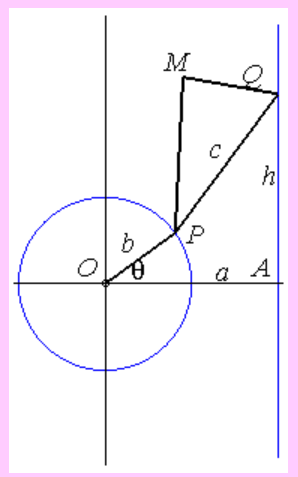
\includegraphics[scale=0.75]{images/SliderCrankMechanismCurve.png}
    \caption{Schéma représentant le mouvement d'un point $M$ sur une bielle qui tourne autour d'un point $O$ avec un angle $\theta$}
    \label{fig:BielleBerard}
\end{figure}

En variant les paramètres, il est possible d'obtenir différents modèles, qui ont ensuite été testés sur SALOME. Les figures \ref{fig:ParamFan1}, \ref{fig:ParamFan2}, \ref{fig:ParamFan3}, \ref{fig:ParamFan4} et \ref{fig:ParamFan5} montrent les résultats de ces tests.

\begin{figure}[H]
    \centering
    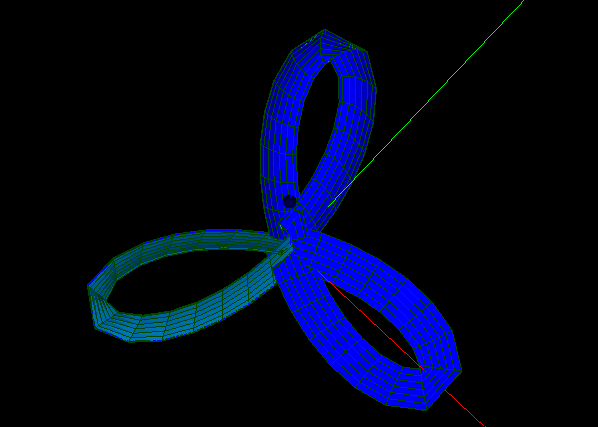
\includegraphics[scale=0.75]{images/ParametricEquation-L0-T0.png}
    \caption{Hélice toroïdales générés avec les paramètres $L=0$, $\theta=0$, $N=3$ et $h=2$}
    \label{fig:ParamFan1}
\end{figure}

\begin{figure}[H]
    \centering
    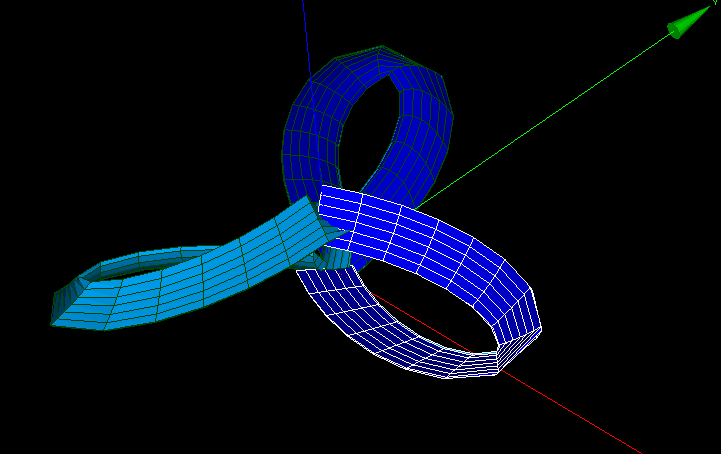
\includegraphics[scale=0.75]{images/ParametricEquation-L0p5.png}
    \caption{Hélice toroïdales générés avec les paramètres $L=0.5$, $\theta=0$, $N=3$ et $h=2$}
    \label{fig:ParamFan2}
\end{figure}

\begin{figure}[H]
    \centering
    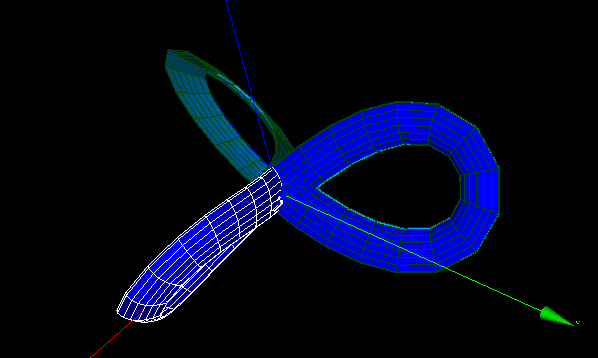
\includegraphics[scale=0.75]{images/ParametricEquation-L0-T0p5.png}
    \caption{Hélice toroïdales générés avec les paramètres $L=0$, $\theta=\frac{\pi}{2}$, $N=3$ et $h=2$}
    \label{fig:ParamFan3}
\end{figure}

\begin{figure}[H]
    \centering
    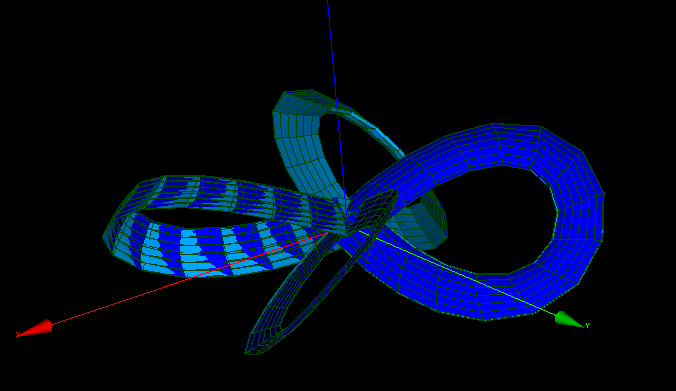
\includegraphics[scale=0.75]{images/ParametricEquation-L0-T0-B4.png}
    \caption{Hélice toroïdales générés avec les paramètres $L=0$, $\theta=\frac{\pi}{2}$, $N=4$ et $h=2$}
    \label{fig:ParamFan4}
\end{figure}

\begin{figure}[H]
    \centering
    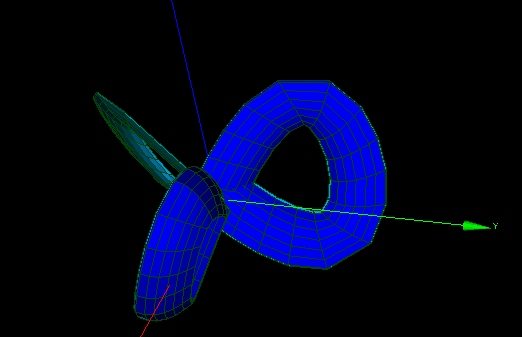
\includegraphics[scale=0.75]{images/ParametricEquation-L0-T0-h1.png}
    \caption{Hélice toroïdales générés avec les paramètres $L=0$, $\theta=\frac{\pi}{2}$, $N=3$ et $h=1$}
    \label{fig:ParamFan5}
\end{figure}

\vspace{1cm}

Ces équations, bien que permettant de varier les paramètres, ne permettent pas de varier la largeur des pales. Or, les pales générées par ces équations sont trop fines pour le ventilateur d'une PAC. Il a donc fallu trouver une autre équation permettant de varier la largeur des pales. Cependant, le manque de temps a empêché de trouver une telle équation. C'est pourquoi, il a fallu encore corriger la roadmap comme mentionné dans la section \ref{sec:Roadmap} pour passer à un autre modèle généré entièrement sur SALOME.

\subsection{Hélice toroïdale adaptée à une pompe à chaleur en CAO}

\label{sec:HeliceToroCAD2}

\hypertarget{Modele4}{Pour} créer ces hélices toroïdales, il faut:

\begin{itemize}
    \item Une courbe guide
    \item Un profil de départ et d'arrivée
    \item Des profils transverses intermédiaires
\end{itemize}

La courbe guide peut être générée en utilisant les barycentres des profils. Donc il faut se concentrer sur les profils. En particulier, il est nécessaire d'avoir des pales très larges au milieu et très fines au bout. La figure \ref{fig:Profile} montre le résultat souhaité.

\begin{figure}[H]
    \centering
    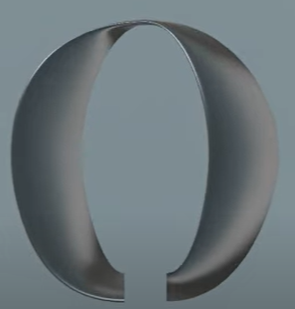
\includegraphics[scale=0.75]{images/Large_Toroidal.png}
    \caption{Vue du dessus d'une pale de l'hélice toroïdale}
    \label{fig:Profile}
\end{figure}

Pour donner cette forme aux pales, des profils NACA pour les pales intermédiaires ont été utilisés. Un profil NACA est un profil aérodynamique. Il est défini par 4 nombres MPXX où:

\begin{itemize}
    \item M définit la cambrure maximale en pourcentage de la corde
    \item P définit le point de cambrure maximale par rapport au bord d'attaque en pourcentage de la corde
    \item XX définissent l'épaisseur maximale du profil en pourcentage de la corde
\end{itemize}

La corde est la distance entre le bord d'attaque et le bord de fuite. Le bord d'attaque est le bord de la pale qui est en contact avec le fluide. Le bord de fuite est le bord de la pale qui est opposé au bord d'attaque. La figure \ref{fig:NACAProfile} montre un schéma représentant un profil NACA.

\begin{figure}[H]
    \centering
    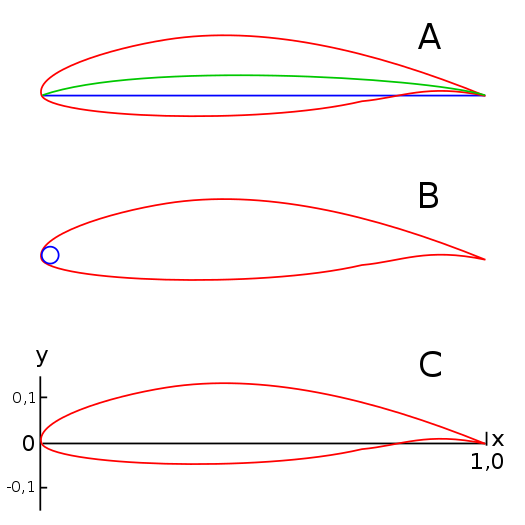
\includegraphics[scale=0.75]{images/NACA_Profile.png}
    \caption{Schéma représentant un profil NACA - A — Ligne bleue : corde. Ligne verte : cambrure moyenne en ligne. B — Premier rayon de bord. C — Coordonnées xy pour la géométrie du profil (corde = axe x; la ligne de l'axe Y sur ce bord d'attaque)}
    \label{fig:NACAProfile}
\end{figure}

Pour générer de tels profils, aucun algorithme permettant de générer ces profils ne sera utilisé. En effet, il existe des sites permettant de générer des profils NACA. Le site suivant: \url{http://airfoiltools.com/search/index} a été utilisé. Il permet d'accéder à une base de données de profils NACA. Maintenant, il est possible de générer une hélice toroïdale. La figure \ref{fig:Toroidal} montre le résultat de l'extrusion d'un profil NACA le long d'une courbe guide.

\begin{figure}[H]
    \centering
    \subfigure[Image 1]{
        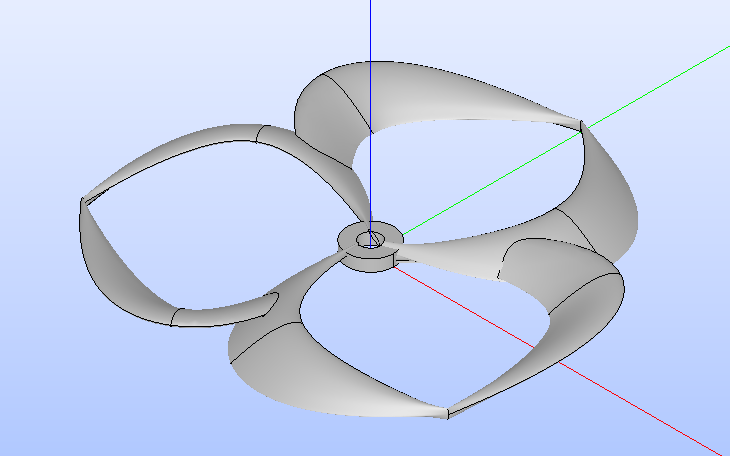
\includegraphics[scale=0.75]{images/ToroidalNACAcad.png}
        \label{fig:Toroidal}
    }
    \hspace{1cm}
    \subfigure[Image 2]{
        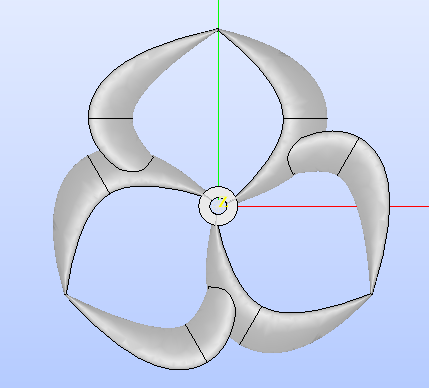
\includegraphics[scale=0.75]{images/ToroidalNACAcad_TopView.png}
        \label{fig:ToroidalTopView}
    }
    \caption{Hélice toroïdale générée sur SALOME}
    \label{fig:Toroidalfan}
\end{figure}

Pour avoir une hélice toroïdale, il faut créer une seule pale et ensuite appliquer une rotation de $\frac{360}{N}$ degrés où $N$ est le nombre de pales. Il faut aussi faire attention à gérer les intersections entre les pales.

Maintenant, pour enlever les irrégularités au bout de la pale, il faut créer une variante de cette hélice avec une courbe guide plus lisse au bout en contrôlant les tangentes de la courbe guide. En effet, la courbe guide est générée avec une interpolation par B-spline. Une B-spline est une courbe paramétrique définie par des points de contrôle (Ici les barycentres des profils) et des vecteurs tangents au début et à la fin de la courbe. La figure \ref{fig:ToroidalVariation} montre le résultat obtenu.

\begin{figure}[H]
    \centering
    \subfigure[Image 1]{
        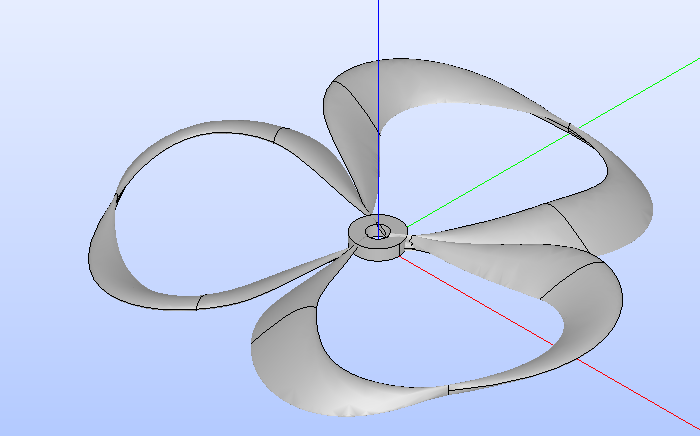
\includegraphics[scale=0.75]{images/ToroidalNACAcad_Smooth.png}
        \label{fig:ToroidalVariation}
    }
    \hspace{1cm}
    \subfigure[Image 2]{
        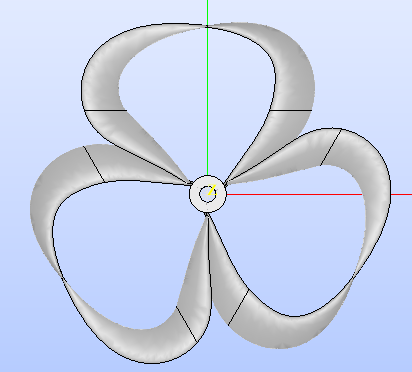
\includegraphics[scale=0.75]{images/ToroidalNACAcad_Smooth_TopView.png}
        \label{fig:ToroidalVariationTopView}
    }
    \caption{Hélice toroïdale générée sur SALOME et lissée au bout de la pale}
    \label{fig:ToroidalfanVariation}
\end{figure}

Cependant, ces courbes ont un défaut majeur, elles ne sont pas lisses à certains endroits. En particulier, le modèle ci-dessus \ref{fig:ToroidalVariation} présente des irrégularités en dessous du ventilateur. Pour remédier à ça, il faut faire attention à ce que chaque profil transverse utilise le même nombre de points. Il est obligatoire de procéder ainsi car l'algorithme d'extrusion de SALOME crée des discontinuités $\mathcal{C}^1$ à chaque changement de nombre de points. La figure \ref{fig:CADNormal} montre le résultat obtenu.

\begin{figure}[H]
    \centering
    \subfigure[Image 1]{
        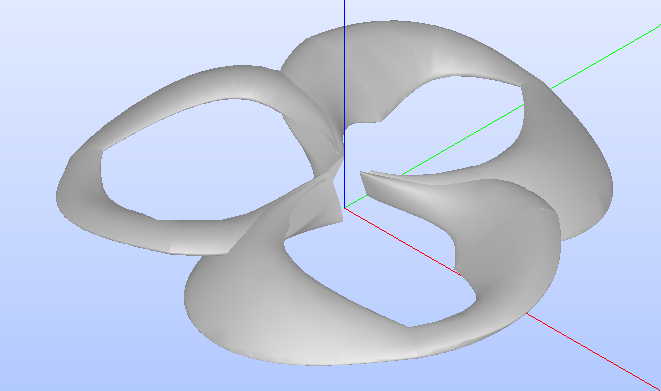
\includegraphics[scale=0.75]{images/CAD_Normal_Oblique_View.png}
        \label{fig:CADNormal}
    }
    \hspace{1cm}
    \subfigure[Image 2]{
        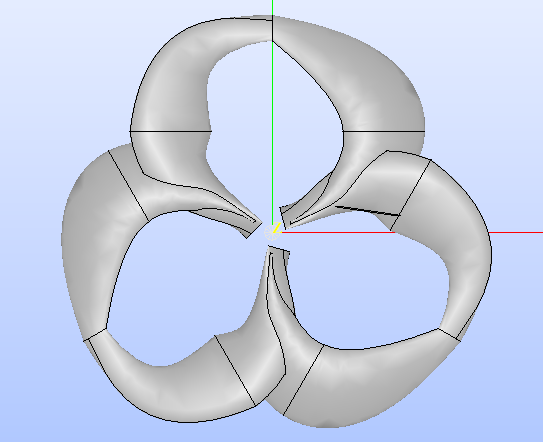
\includegraphics[scale=0.75]{images/CAD_Normal.png}
        \label{fig:CADNormalTopView}
    }
    \caption{Hélice toroïdale générée et lissée sur SALOME}
    \label{fig:Toroidalfan}
\end{figure}

Pour respecter la roadmap, il a également fallu générer des variations avec une profondeur de pale plus importante, ainsi qu'une variation avec un profil intermédiaire plus fin. Les figures \ref{fig:CADDeeper} et \ref{fig:CADNACA} montrent les résultats obtenus.

\begin{figure}[H]
    \centering
    \subfigure[Image 1]{
        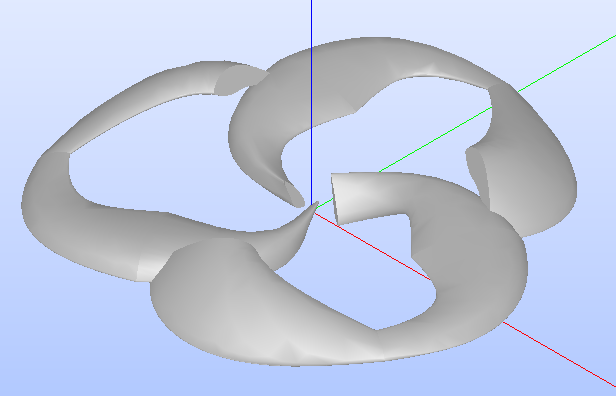
\includegraphics[scale=0.75]{images/CAD_Deeper_Oblique_View.png}
        \label{fig:CADDeeper}
    }
    \hspace{1cm}
    \subfigure[Image 2]{
        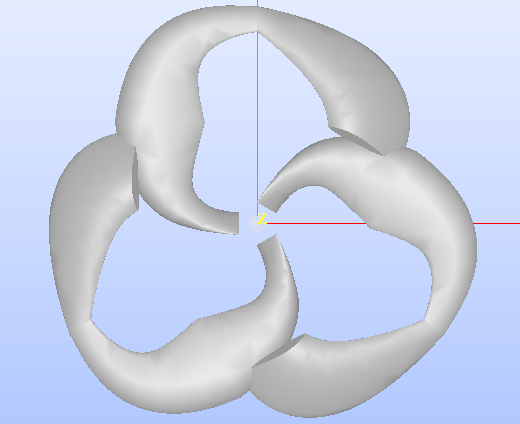
\includegraphics[scale=0.75]{images/CAD_Deeper.png}
        \label{fig:CADDeeperTopView}
    }
    \caption{Variante plus profonde de l'hélice toroïdale générée sur SALOME}
\end{figure}

\begin{figure}[H]
    \centering
    \subfigure[Image 1]{
        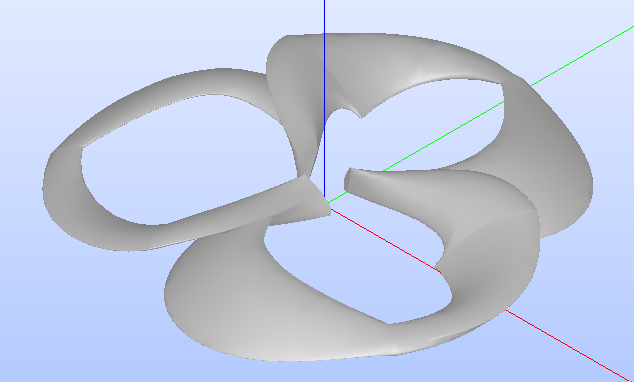
\includegraphics[scale=0.75]{images/CAD_NACA_Variation_Oblique_View.png}
        \label{fig:CADNACA}
    }
    \hspace{1cm}
    \subfigure[Image 2]{
        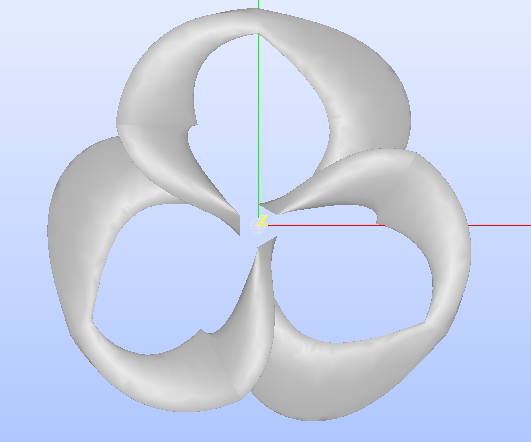
\includegraphics[scale=0.75]{images/CAD_NACA_Variation.png}
        \label{fig:CADNACATopView}
    }
    \caption{Variante avec un profil intermédiaire plus fin de l'hélice toroïdale générée sur SALOME}
\end{figure}

Malgré ces améliorations, il y a toujours des irrégularités sur les courbes. Les irrégularités sont flagrantes sur le modèle \ref{fig:CADNACA}. Mais le manque de temps a empêché de trouver une solution pour générer des courbes plus lisses.

\subsection{Tableau comparatif des différents modèles générés}

Comme plusieurs modèles d'hélices toroïdales ont été générés, il faut dresser un tableau comparatif pour pouvoir choisir le modèle le plus adapté. Le tableau \ref{tab:my_label} montre les avantages et les inconvénients de chaque modèle.

\begin{table}[H]
    \centering
    \begin{tabular}{|c|c|c|}
        \hline
        & \textbf{Avantages} & \textbf{Inconvénients} \\
        \hline
        \hyperlink{Modele1}{\textbf{Modèle 1}} & \begin{tabular}{@{}c@{}}- Facile à générer \\ - Possibilité de générer des hélices \\ avec des profils NACA\end{tabular} & \begin{tabular}{@{}c@{}}- Difficile de varier \\ les paramètres \\ - Les profils transverses ne sont pas \\ assez larges pour un ventilateur de PAC\end{tabular} \\
        \hline
        \hyperlink{Modele2}{\textbf{Modèle 2}} & \begin{tabular}{@{}c@{}}- Facile à générer \\ - Les intersections entre les hélices \\ sont facilement automatisables\end{tabular} & \begin{tabular}{@{}c@{}}- On ne peut pas varier \\ les paramètres \\ - Les profils transverses n'ont pas un profil NACA\end{tabular} \\
        \hline
        \hyperlink{Modele3}{\textbf{Modèle 3}} & \begin{tabular}{@{}c@{}}- Facile à générer \\ - Possibilité de varier \\ les paramètres \end{tabular} & \begin{tabular}{@{}c@{}}- Difficile de varier \\ la largeur des pales \\ - Les intersections entre les hélices \\ doivent être gérées au cas pas cas \end{tabular} \\
        \hline
        \hyperlink{Modele4}{\textbf{Modèle 4}} & \begin{tabular}{@{}c@{}} - Possibilité de varier \\ les paramètres \\ - Possibilité de varier \\ la largeur des pales\end{tabular} & \begin{tabular}{@{}c@{}}- Irrégularité dans le ventilateur \\ - Les intersections entre les hélices \\ doivent être gérées au cas pas cas\end{tabular} \\
        \hline
    \end{tabular}
    \caption{Tableau comparatif des différents modèles générés}
    \label{tab:my_label}
\end{table}

\section{Conclusion}

\subsection{Pistes d'amélioration}

À partir de tout ce qui a été vu, plusieurs idées d'amélioration du modèle peuvent être dressées:

- Travailler sur de nouvelles équations pour générer des courbes guides: Vers la fin du projet, une équation permettant de générer des courbes guides avec des pales très larges au milieu et très fines au bout a été trouvé. Cependant, il n'y a pas eu assez de temps pour tester cette équation. Il faudrait donc tester cette équation pour voir si elle permet de générer des hélices toroïdales satisfaisantes.

- Générer des courbes plus lisses en CAO: Bien qu'il soit possible de générer des courbes plus lisses, ils restent des endroits irréguliers. Il faudrait donc essayer de trouver une solution pour générer des courbes totalement lisses en CAO.

\subsection{Bilan}

Pour conclure, des premiers modèles d'hélices toroïdales ont pu être générés. Ces modèles sont satisfaisants car ils permettent de varier les paramètres géométriques.

Cependant, les modèles sont irréguliers à certains endroits. Il faut donc trouver une solution pour générer des courbes plus lisses en CAO.

\section{Bibliographie}

\begin{itemize}
    \item Toroidal propeller MIT \href{https://www.ll.mit.edu/sites/default/files/other/doc/2023-02/TVO_Technology_Highlight_41_Toroidal_Propeller.pdf}{[1]}
    \item Mathematical expression method for geometric shape of toroidal propeller, YE Liyu, WANG Chao, SUN Cong, GUO Chunyu, 2023 \href{http://www.ship-research.com/cn/article/doi/10.19693/j.issn.1673-3185.03419}{[2]}
    \item Toroidal propeller generator \href{https://github.com/RaulBejarano/Ultimate-Toroidal-Propeller-Generator}{[3]}
    \item P. RATHOA - Private Communication [4]
    \item Trifolium régulier \href{https://mathcurve.com/courbes2d/trifoliumregulier/trifoliumregulier.shtml}{[5]}
    \item Courbe de la bielle de Bérard \href{https://mathcurve.com/courbes2d/bielledeberard/bielledeberard.shtml}{[6]}
    \item Profil NACA \href{https://fr.wikipedia.org/wiki/Profil_NACA}{[7]}
    \item Toroidal Propeller Tutorial in Fusion 360 for FPV Drones \href{https://www.youtube.com/watch?v=UUPffl7JxKw}{[8]}
\end{itemize}

\end{document}